%%%%%%%%%%%%%%%%%%%%%%%%%%%%%%%%%%%%%%%%%%%%%%%%%%%
%
%  New template code for TAMU Theses and Dissertations starting Fall 2012.  
%  For more info about this template or the 
%  TAMU LaTeX User's Group, see http://www.howdy.me/.
%
%  Author: Wendy Lynn Turner 
%	 Version 1.0 
%  Last updated 8/5/2012
%
%%%%%%%%%%%%%%%%%%%%%%%%%%%%%%%%%%%%%%%%%%%%%%%%%%%
%%%%%%%%%%%%%%%%%%%%%%%%%%%%%%%%%%%%%%%%%%%%%%%%%%%%%%%%%%%%%%%%%%%%%%
%%                           SECTION III
%%%%%%%%%%%%%%%%%%%%%%%%%%%%%%%%%%%%%%%%%%%%%%%%%%%%%%%%%%%%%%%%%%%%%

\chapter{\uppercase{State of the art}}

\section{Introduction}
Autonomous air vehicles (a.k.a Drones) have been an area of research that has been of great interest for many years. Currently, the most prestigious universities and research centers, both private and public, are exploring, researching, and developing autonomous air vehicles using deep learning. These platforms have been used to investigate in areas ranging from non-linear controls, multivariable controls, navigation, trajectory planning to the detection and visual tracking of targets.

One of the most remarkable UAVs among the wide variety of autonomous air vehicles, are autonomous helicopters. They are easy to maneuver and possess properties that make them very suitable for inspection and monitoring tasks. Their inherent ability to fly at low speeds, laterally or longitudinally, to make stationary flights, and maneuvering in tight spaces make them ideal vehicles for such tasks. Typical missions require the helicopter to fly at low speed or to maintain a  stationary flight position next to a region/object of interest. This proximity in the flight is done using the inertial measurements and/or measures of a GPS, which limits the flight to a previous knowledge of the global position of the object or to a pre-programmed route of coordinates. A vision system that can, in real time, control the helicopter in an arbitrary path is not subject to these limitations, and on the contrary combined with other sensors can increase the precision in the flights near objects of interest, allowing to know the relative position of the vehicle with respect to the region/object Of interest.

The development of an autonomous air vehicle  guided by computer vision requires research in areas such as control, state estimation, visual control, and analysis, detection and tracking of objects through computer vision. The following work focuses on the visual control, the analysis and detection of objects exploring the possibilities of using computer vision to control the position of an autonomous air vehicle with respect to an object of interest, making use of previous works in the area of control of UAVs and computer vision. The literature review presented in this section refers to controlling and modeling of autonomos air vehicles, with a special focus on object detection, and tracking and its possible application to visual control on UAVs. Throughout next chapter, We will further present an extensive review of the current state of the art on controlling UAVs using computer vision. For an excellent bibliography on control and modeling of unmanned aerial vehicles, the reader is referred to [Saripalli et al., 2003b], [Shim et al., 1998], [Conway, 1995], [Montgomery, 1999].
  

\begin{figure}[h!]
\centering
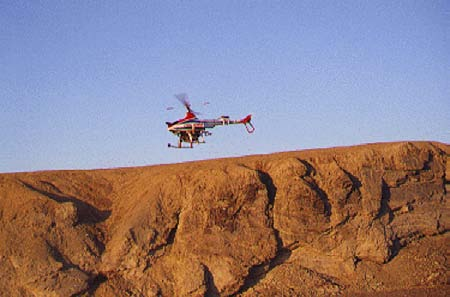
\includegraphics[scale=0.9]{figures/helicopter.png}
\caption{Carnegie Mellon University Helicopter: Autonomous Helicopter Project}
\label{automonous_drone}
\end{figure}

\section{Computer Vision in UAVs}

Computer vision is one of the most important sensors in robotics. In previous years, the complexity, computational cost, high bandwidth requirements had been the major obstacles to robust servo visual control. With the introduction of high-speed processors, low-cost digital cameras and faster graphics cards, real-time visual processing, visual servo control, and servo manipulator control has become a reality.

When one refers to visual control, in particular to visual control in autonomous aerial vehicles, one makes reference to the use of visual information obtained from image processing in order to control speed, absolute or relative position, and orientation of an aerial robot (UAV).

One of the first autonomous helicopters, figure \ref{automonous_drone}, guided by computer vision is described in [Amidi, 1996]. This vehicle combines the GPS readings with a vision system, in order to increase the precision of the state estimate for navigation. The vision system consists of a DSP (Digital Signal Processor) that provides position, velocity and attitude measurements at frequencies of the order of 10ms, which combined with the GPS and IMU (Inertial Measurement Unit)  readings increases the accuracy in estimating the attitude and position of the helicopter. 

[Bosse, 1997] focuses on the use of a camera as an additional sensor for the navigation of an autonomous helicopter. Given a sequence of images taken by a camera the estimate of 3D movement of the camera is achieved. This estimate is then merged with inertial information which is applied to help the UAV during landing process. Visual control has also been applied to miniature vehicles, in the case of a four-rotor helicopter (HUX-4) [Altug, 2003], [Altug et al., 2005] where vision is used to determine the arrangement(disposicion) of the helicopter and for the detection of objects on land. In the case of a miniature aircraft [Causey, 2003] the detection and location of the horizon is used for the lateral control of a mini UAV.

Zhang [Zhang, 2000] used an on-board camera to detect and follow a colored circle in order to control an airship. The planning of the trajectory is done in the plane of the image, which eliminates the calibration and saves computational cost. However the visual control is done by introducing the dynamics of the system (airship) while in the visual processing.

In the area of autonomous landing based on vision, recently in [Merz et al., 2004] the detection of a known pattern using computer vision and the fusion of this information with the inertial measures allows this helicopter to land in case of non-availability of GPS. In [Johnson et al., 2005] computer vision techniques are used to recover and detect safe areas for landing on an unknown terrain. Previously, artificial vision was used to autonomously land a helicopter using two different strategies [Saripalli et al., 2003a] and [Shakernia et al., 1999], but with the particularity of computer vision as the main source of information.

In the case of 3D navigation based on Habrar [Hrabar, 2006], it proposes an obstacle avoidance technique based on computer vision combining optical flow and stereoscopic vision. Experiments demonstrate the advantages of combining both techniques, which in turn combined with a path planner based on probabilistic maps allows the navigation of a stand-alone helicopter in urban environments.

This chapter has presented an overview of current works and developments in autonomous air vehicles, with particular emphasis on autonomous helicopters. The rapid development of this technology is making the state of the art progress vertiginously finding new developments and applications every day, some because of their private nature are not publicly documented. Although, the subject of helicopter control has been well studied and is being considered solved, this is not the case when using computer vision for visual control. The high requirements of reliability and robustness necessary by UAV control urges for new developments and techniques for computer vision that satisfy these demands.


\section{OpenCV}

Artificial vision is one of the main scientific disciplines when it comes to reproducing what human beings can perceive through their own physical senses in a computer. The analysis and the processing of images are one of the methods that form the basis of the artificial vision. In computing there are several techniques such as pattern search, image filtering, or projective integrals  that require complex algorithms and considerable computational effort.

One of the most used resources in the field of artificial vision is OpenCV. This is a free software library that includes various pieces of code written in C ++, C, Python, Java and Matlab. OpenCV is capable of producing more than 500 algorithms with different functionalities that cover much of the analysis of images and the well-known learning of the machine. It has a modular structure (Figure \ref{opencv_structure}) that facilitates its use when it comes to including libraries in projects. Each module differs to produce a different functionality. The main modules of OpenCV are: core, imgproc, video, calib3d, features2d, objdetect, highgui and gpu.

\begin{figure}[h!]
\centering
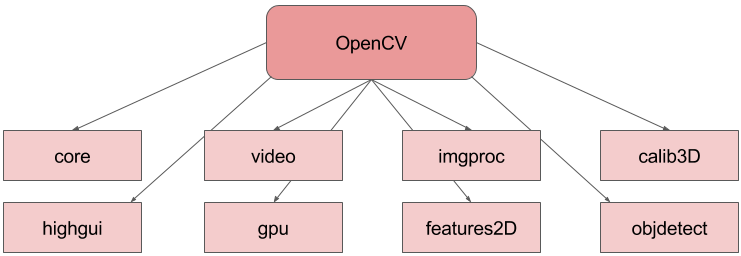
\includegraphics[scale=0.7]{figures/opencv_structure.png}
\caption{Basic components of OpenCV that form the modular structure}
\label{opencv_structure}
\end{figure}

The main objective of OpenCV is to provide tools that help people build programs related to image analysis that are increasingly sophisticated and optimal, as we can see in facial detection methods in the image (Figure \ref{image_processing}).

\begin{figure}[h!]
\centering
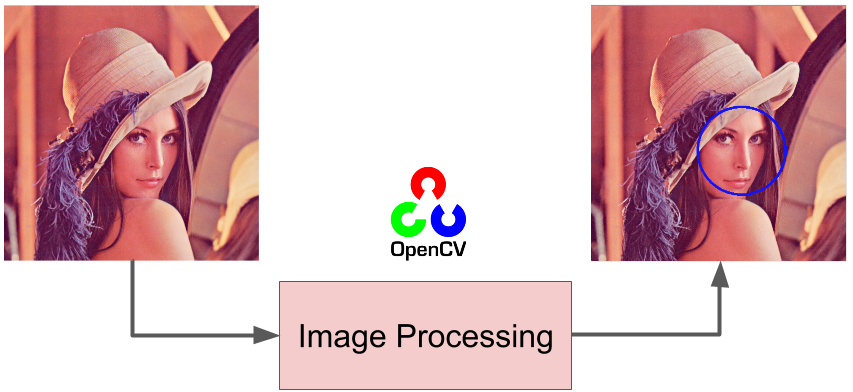
\includegraphics[scale=0.7]{figures/image_processing.png}
\caption{Example of facial detection in OpenCV with Lena Söderberg}
\label{image_processing}
\end{figure}


%\begin{figure}[h]
%\centering
%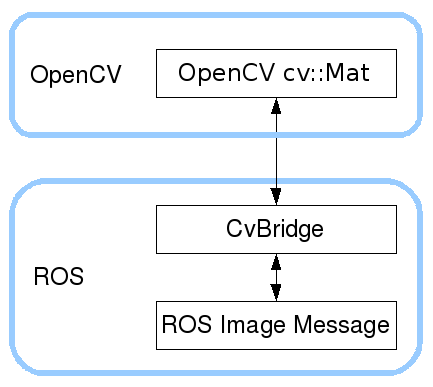
\includegraphics[scale=0.4]{figures/cv_bridge.png}
%\caption{Pipeline from a ROS image to an OpenCV image \cite{ApacheHadoop}}
%\label{HDFSArch}
%\end{figure}

\section{TLD (Tracking-Learning-Detection)}

Tracking-Learning-Detection (TLD), also known as Predator algorithm is a real-time algorithm for the tracking of unknown objects in video streams developed by Zdenek Kalal[28].

The object of interest is defined by a bounding box in a single frame and TLD simultaneously tracks the object, learns its appearance and detects it whenever it appears in the video.
By separating tracking and detection, TLD algorithm outperforms existing adaptive tracking-by-detection methods. Also, a notable reduction in the computing time is achieved by using simple features for object detection.

The TLD framework decomposes the long-term tracking task into three sub-tasks: tracking, learning and detection. Each sub-task is addressed by a single component and they operate simultaneously(see Figure \ref{tld_process}).

\begin{itemize}
\setlength{\itemsep}{-10pt}
\item \textbf{Tracker:}Follows the object through the frames.
\item \textbf{Detector:} Localizes all the appearances that have been observed so far and corrects the tracker if necessary.
\item \textbf{Learning:} Estimates the error and updates it to avoid these error in the future.
\end{itemize}

The TLD work-flow starts with the initialization, which leads to a learning step. 
Then the tracker. The diagram below shows the process:

\begin{figure}[h!]
\centering
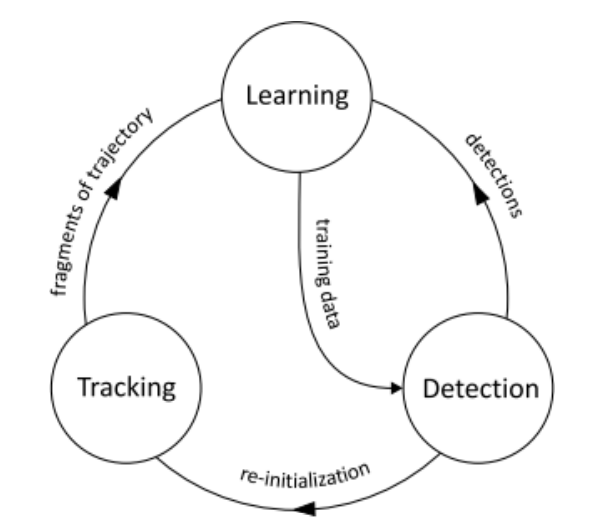
\includegraphics[scale=0.6]{figures/tld_process.png}
\caption{Block diagram of the Tracking Learning Detection algorithm}
\label{tld_process}
\end{figure}


\section{Image Recognition: TensorFlow}

\begin{figure}[h]
\centering

\includegraphics[scale=0.4]{figures/tensorflow_logo.png}
\caption{TensorFlow Logo}
\label{TensorFlow_Logo}
\end{figure}

Image recognition is a very powerful tool that is performed through automated learning. In general, it is a process that requires a very high computational complexity because it has to simulate a cognitive stimulation that exercises sensorial perception in humans, similar to gnosia.

In recent years, There has been tremendous progress in tackling these difficulties. In particular, Google has developed an automatic learning tool that uses a neural convolution network which has come to produce the same results or even improve them in comparison to human visual recognition tasks.

This tool is called TensorFlow, figure  \ref{TensorFlow_Logo}, released on the 15th of November 2015 by Google, TensorFlow is an open source library TensorFlow is an open source library that is based on a neural network system. This means that it can relate several data on the network simultaneously, in the same way as the human brain does.

%Released on the 15th of November 2015 by Google, TensorFlow is an open source library that is based on a neural network system. This means that it can relate several data on the network simultaneously, in the same way as the human brain does. 

Tensorflow's  automatic learning system specializes in voice recognition, text recognition, and image recognition. For example, you can recognize several words in the alphabet because it relates letters and phonemes. \\ Another case is that of images and texts that can be related to each other quickly thanks to the association capacity of the neural network system. According to Google, TensorFlow can be very useful for health, insurance and automotive commercial sectors. Since it released the code, several companies, Universities, and researchers use the software or have relied on it to develop applications.

\begin{figure}[h]
\centering
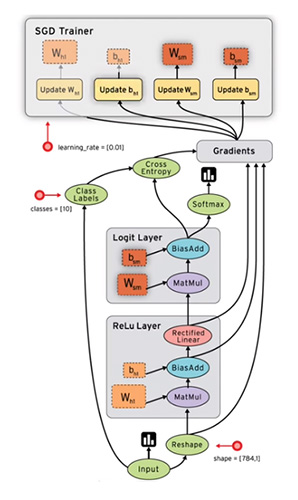
\includegraphics[scale=0.5]{figures/TensorFlow-graph.jpg}
\caption{TensorFlow graph}
\label{TensorFlow-graph}
\end{figure}

\section{Inception-V3}

Inception-v3 is a version of a TensorFlow model for image recognition, trained from the ImageNet 7 neural network. Inception-v3 has the ability to classify images into more than 1000 classes according to the degree of similarity it encounters.

This model first identifies the main characteristics of the image that we want to recognize, obtaining the contours of the figure as a function of its geometry and contrast with the background. Next, an algorithm is in charge of relating the whole geometry obtaining an abstract representation of our figure to classify.

It is at this point when the system decides to make the comparison of our figure with the model that has been trained from images that exist on the web. The model searches the database for a figure to which it corresponds in order to obtain a ranking of 5 probabilities that represent the degree of similarity. The higher the likelihood, the more correct is the classification of the image. This process can be defined as a question-and-answer system, figure \ref{neural_net}, since in order to obtain a reliable answer, all the pixels in the image are analyzed and questions are asked to the model in order to obtain a reliable result based on a logical and intuitive response.

\begin{figure}[!ht]
\centering
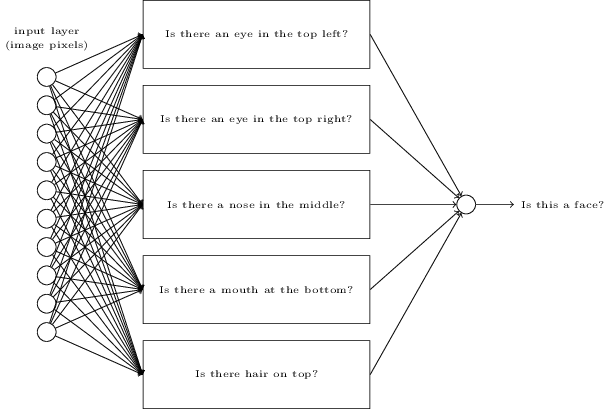
\includegraphics[scale=1.0]{figures/neural_net.png}
\caption{Architecture of a model that uses a neural network for face recognition}
\label{neural_net}
\end{figure}


%%%%%%%%%%%%%%%%%%%%%%%%%%%%%%%%%%%%%%%%%%%%%%%%%%%%%%%
%\subsection{Subsection}

%A table example is going to follow.

%\begin{table}[H]
%\centering
%\caption{This is a table template}
%\begin{tabular}{|l|c|c|c|c|c|}
%\hline
%Product & 1 & 2 & 3 & 4 & 5\\
%\hline
%Price & 124.- & 136.- & 85.- & 156.- & 23.-\\
%Guarantee [years] & 1 & 2 & - & 3 & 1\\
%Rating & 89\% & 84\% & 51\% & & 45\%\\
%\hline
%\hline
%Recommended & yes & yes & no & no & no\\
%\hline
%\end{tabular}
%\label{tab:template2}
%\end{table}
%\subsubsection{This is a subsubsection}


